\documentclass[22pt]{article} 
\usepackage{geometry} 
\usepackage{float} 
\usepackage{graphicx}
\usepackage{caption}
\usepackage{subfigure}
\usepackage{amsmath}
\usepackage{array}
\usepackage{tikz}
\usetikzlibrary{trees}
\usepackage{listings}
\usepackage[framed,numbered,autolinebreaks,useliterate]{mcode}%matlab
\usepackage{algorithm} % 伪代码	
\usepackage{algorithmic}  %伪代码
\renewcommand{\algorithmicrequire}{\textbf{Input:}} 
\renewcommand{\algorithmicensure}{\textbf{Output:}}

\geometry{left=2.0cm,right=2.0cm,top=0.5cm,bottom=0.5cm}
	\author{Mengfan Wang PID:mengfanw} 
	\title{Data Analytics Homework 4} 
\begin{document}
	\maketitle 
	\paragraph{1}
		\subparagraph{a} The 5-nearest neighbors of the triangle point are 3 circles (distances are $1$, $3$, $\sqrt{10}$) and 2 squares (distances are $\sqrt{2}$ and $\sqrt{5}$) according to Euclidean distance. So the test point will be classified as a negative point.

		\subparagraph{b} The 3-nearest neighbors of the triangle point are 1 circles (distance is 1) and 2 squares (distance is 2 and 3) according to Manhattan distance. The weight of circles are $1/1 = 1$, and the weight of squares are $1/4+ 1/9 = 17/36$. So the test point will be classified as a negative point.

	\paragraph{2} H1: When H1 is the first weak classifier, the last two instances are classified wrongly. $\alpha_1 = \frac{1}{2}log(\frac{1-0.2}{0.2}) = 0.69$. For those classified wrongly, $w_i = 0.1\times e^{0.69}=0.199$, and for those classified correctly, $w_i = 0.1\times e^{-0.69}=0.050$. Therefore, the weights of the first eight eight instances are 0.050 and those of the last two instances are 0.199.\\[1ex]
	H2: When H2 is the first weak classifier, the first three instances and the $8_{th}$ instance are classified wrongly. $\alpha_1 =  \frac{1}{2}log(\frac{1-0.4}{0.4}) = 0.20$. For those classified wrongly, $w_i = 0.1\times e^{0.20}=0.122$, and for those classified correctly, $w_i = 0.1\times e^{-0.69}=0.082$. Therefore, the weights of the first three and the $8_{th}$ instances are 0.122 and those of others are 0.082.\\[1ex]
	H3: When H3 is the first weak classifier, the $9_{th}$ instance is classified wrongly. $\alpha_1 =  \frac{1}{2}log(\frac{1-0.1}{0.1}) = 1.10$. For those classified wrongly, $w_i = 0.1\times e^{1.10}=0.300$, and for those classified correctly, $w_i = 0.1\times e^{-0.69}=0.033$. Therefore, the weights of the $9_{th}$ instance is 0.300 and those of others are 0.033.  

	\paragraph{3}
		\subparagraph{1} Because all the items in $X$ are independent, we have:
		\begin{equation}
			P(X) = \Pi_iP(x_i)
		\end{equation}
		So,
		\begin{equation}
			cosine(X) = \frac{P(X)}{\sqrt{\Pi_iP(x_i)}} = \sqrt{\Pi_iP(x_i)}
		\end{equation}

		\subparagraph{2} The answer is non-monotone. Suppose two situations: 

		Firstly, suppose the transactions are $\{\{a,b,c\},\{a,b\}\}$. $cosine(\{a,b\}) = P(\{a,b\})/ \sqrt{P(\{a\})P(\{b\})} = 1$, and $cosine(\{a,b,c\}) = P(\{a,b,c\})/ \sqrt{P(\{a\})P(\{b\})P(\{c\})} = 0.707$. In this situation the measure is decreasing.

		Secondly, suppose the transactions are $\{\{a,b,c\},\{a\},\{b\},\{c\}\}$. $cosine(\{a,b\}) = P(\{a,b\})/ \sqrt{P(\{a\})P(\{b\})} = 0.5$, and $cosine(\{a,b,c\}) = P(\{a,b,c\})/ \sqrt{P(\{a\})P(\{b\})P(\{c\})} = 0.707 $. In this situation the measure is increasing.



 		\subparagraph{3} Firstly of all, a proposition of cosine measure needs to be proved: For any itemset $S = \{x_1,x_2\dots x_i\}$, while $P(x_1) \geq P(x_2) \geq \dots P(x_i)$, $\forall G \subset S $, $cosine(G\cup\{x_i\})\leq cosine(S)$, because:
 		\begin{align}
 		 cosine(S) & = \frac{P(S)}{\sqrt{\Pi_{j\in S}P(x_j)}}\\
 		 & \leq \frac{P(x_i)}{\sqrt{\Pi_{j\in S}P(x_j)}}
 		\end{align}
 		and,
 		\begin{align}
 		cosine(G\cup\{x_i\}) &  = \frac{P(G\cup\{x_i\})}{\sqrt{\Pi_{j\in G}P(x_j)}}\\ 
 		& \leq \frac{P(x_i)}{\sqrt{\Pi_{j\in G}P(x_j)}}\\
 		& \leq \frac{P(x_i)}{\sqrt{\Pi_{j\in S}P(x_j)}}
 		\end{align}
 		Define $sup\ cosine(S) = \frac{P(x_i)}{\sqrt{\Pi_{j\in S}P(x_j)}}$, while $x_i$ is the last item in $S$. For any subset $G$ of $S$ with $x_i$, we have $cosine(G) \leq sup\ cosine(G) \leq sup\ cosine(S)$. For example, $cosine(\{e\}) \leq sub\ cosine(\{e\}) \leq sub\ cosine(\{a,b,e\}) \leq sub\ cosine(\{a,b,c,d,e\})$. The algorithm is:


 		\begin{algorithm}
			\begin{algorithmic}[1]
			\REQUIRE The database $\mathcal{D}$ and the itemset $X = \{x_1,x_2\dots x_d\}$
			\ENSURE Itemsets whose cosine similarity $\geq \tau$
			\FOR {i = 1 to d-1}
			\STATE Set $G = \{x_1, x_2,\dots x_i\}$
			\STATE Compute $sup\ cosine(G\cup \{x_{i+1}\}) = \frac{P(x_{i+1})}{\sqrt{(\Pi_{j\in G}P(x_j))P(x_{i+1})}}$
			\IF {$sup\ cosine(G\cup \{x_{i+1}\}) < \tau$ }
			\STATE Delete $G\cup \{x_{i+1}\}$ and all subsets of $G\cup \{x_{i+1}\}$ with item $x_{i+1}$. Continue to compute the next set or subset. 
			\ELSE
			\STATE Label $G$.
			\ENDIF
			\STATE If $G$ is a subset of $\{x_1, x_2,\dots x_i\}$ and there are other subsets with the same number of items, choose one as $G$; else, choose one subset with one less items of $\{x_1, x_2,\dots x_i\}$  as $G$. Deleted subsets and labeled subsets can't be chosen. Go back to step 3. If no subsets can be chosen, continue to the next loop.
			\ENDFOR
			\STATE Computer the cosine similarity of all reserved itemsets and determine to reserve them or delete them.
			\end{algorithmic}
			\end{algorithm}

	\paragraph{4}
		\subparagraph{1}
		The hash tree is:\\
		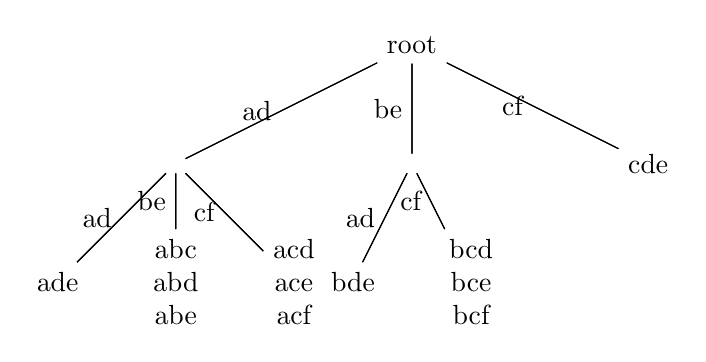
\begin{tikzpicture}[level distance=1.5cm,
		  level 1/.style={sibling distance=3cm},
		  level 2/.style={sibling distance=1.5cm}]
		  \node (root){root}
		    child {node (ad1){}
		      child {node (ad2){ade}}
		      child {node[align = center] (be2){abc\\abd\\abe}}
		      child {node[align = center] (cf2){acd\\ace\\acf}}
		    }
		    child {node(be1) {}
		      child {node (ad3) {bde}}
		      child {node[align = center](cf3) {bcd\\bce\\bcf}}
		    }
		    child {node(cf1) {cde}
		   };

		   \draw[left](root) -- node  {ad} (ad1);
		   \draw[left](root) -- node  {be} (be1);
		   \draw[left](root) -- node  {cf} (cf1);
		   \draw[left](ad1) -- node  {ad} (ad2);
		   \draw[left](ad1) -- node  {be} (be2);
		   \draw[left](ad1) -- node  {cf} (cf2);
		   \draw[left](be1) -- node  {ad} (ad3);
		   \draw[left](be1) -- node  {cf} (cf3);
		\end{tikzpicture}

		\subparagraph{2} The subsets of this transaction are $\{a,b,d\}$, $\{a,b,e\}$, $\{a,b,f\}$, $\{a,d,e\}$, $\{a,d,f\}$, $\{a,e,f\}$, $\{b,d,e\}$, $\{b,d,f\}$, $\{b,e,f\}$, and $\{d,e,f\}$. They can be hashed into $root \rightarrow ad \rightarrow ad$, $root \rightarrow ad \rightarrow be$, $root \rightarrow be \rightarrow ad$, $root \rightarrow be \rightarrow be$, totally 4 leaf nodes.

		\subparagraph{3}
		 $\{a,b,c,d\}$, $\{a,b,c,e\}$, $\{a,b,c,f\}$, $\{a,b,d,e\}$, $\{a,b,d,f\}$, $\{a,b,e,f\}$, $\{a,c,d,e\}$, $\{a,c,d,f\}$, $\{a,c,e,f\}$, $\{a,d,e,f\}$, $\{b,c,d,e\}$,  $\{b,c,d,f\}$,  $\{b,c,e,f\}$,  $\{b,d,e,f\}$,  $\{c,d,e,f\}$.

		\subparagraph{4} If a 4-itemset is frequent, all of its 3-item subsets must be frequent. So the list is: $\{a,b,c,d\}$,  $\{a,b,c,e\}$, $\{a,b,d,e\}$, $\{a,c,d,e\}$, $\{b,c,d,e\}$.

		\subparagraph{5} It's possible, and the only possible transaction is $\{a,b,c,d,e\}$, because all of its 3-itemsets are frequent. 
		
	\paragraph{5} 
	\subparagraph{1.a}
	For a given $k$-itemset $X$, there are $d-k$ discriminative rules;

	For a given number $k$, there are $\binom{d}{k}$ left-side itemsets. So the maximum number of rules is:
	\begin{align}
		& \sum\limits_{k = 1}^{d-1}[\binom{d}{k}(d-k)]\\
		= & d \sum\limits_{k = 1}^{d-1} \binom{d}{k} - \sum\limits_{k = 1}^{d-1} k \binom{d}{k}]\\
		= & d \sum\limits_{k = 1}^{d-1} \binom{d}{k} - d\sum\limits_{k = 1}^{d-1}  \binom{d-1}{k-1}\\
		= & d (2^d-2) - d(2^{d-1} -1 )\\
		= & d(2^{d-1}-1)
	\end{align}

	\subparagraph{1.b} Because $y$ is not included in $X$, for a given frequent $k$-itemset $X$, the maximum number of discriminative rules that can be extracted is $d-k$.

	\subparagraph{1.c} I don't think the support of subsets of $X$ can guarantee $X$ will generate rules with confidence $\geq minconf$.

	\subparagraph{2.a} The answer is same as part 1.a, $d(2^{d-1}-1)$. 

	\subparagraph{2.b} The answer is same as part 1.b, $d-k$.

	\subparagraph{2.c} For any $X$ and $y$ ($y\notin X$), we have:
	\begin{align}
		conf(y\rightarrow X) = \frac{P(X,y)}{P(y)} \leq \frac{P(X)}{P(y)} \leq \frac{P(X)}{P(x_m)},
	\end{align}
	while $x_m$ is the item which not in $X$ and has the minimum subscript. Define $sup\ conf(X) = \frac{P(X)}{P(x_m)}$, which satisfies Apriori principle. Suppose $X'$ is a superset of $X$, we have $P(X) \geq P(X')$ and $P(x_m) \leq P(x_m')$, so $sup\ conf(X) \geq sup\ conf(X')$. So the algorithm is:

	\begin{algorithm}
			\begin{algorithmic}[1]
			\REQUIRE The database $\mathcal{D}$ and the itemset $X = \{x_1,x_2\dots x_d\}$.
			\ENSURE Characteristic rules whose support $\geq minsup$ and confidence $\geq minconf$.
			\STATE Let k=1
			\STATE Generate frequent itemsets of length 1. (support $\geq minsup$ and $sup\ conf \geq minconf$)
			\REPEAT 
			\STATE Generate length (k+1) candidate itemsets from length k frequent itemsets.
			\STATE Prune candidate itemset contain subsets of length k that are infrequent.
			\STATE Count the support of each candidate by scanning the DB, and find the item for each candidate with least support and not in each candidate.
			\STATE Eliminate candidates that are infrequent, leaving only those that are frequent. (support $\geq minsup$ and $sup\ conf \geq minconf$)
			\STATE k = k + 1
			\UNTIL No new frequent itemsets are identified. 
			\FOR {X = All frequent itemsets}
			\FOR {y = All item not in X }
			\IF {$\frac{P(X)}{P(y)} \geq minconf$}
			\STATE Compute $conf(y\rightarrow X) = \frac{P(X,y)}{P(y)}$. If $conf(y\rightarrow X) \geq minconf$, $y \rightarrow X$ is an associate rule.
			\ELSE
			\STATE Jump to the next outside loop.// If $\frac{P(X)}{P(y)} \leq minconf$, all items after $y$ cannot generate associate rules.
			\ENDIF
			\ENDFOR
			\ENDFOR
			\end{algorithmic}
			\end{algorithm}


	\paragraph{6} 
	\subparagraph{1} The minimum number of maximal frequent itemsets is 1. For example, $\{A,B,C,D,E\}$ is the maximal frequent itemset.

	The maximal number of maximal frequent itemsets is 10. For example, all 2-itemsets are maximal frequent itemsets.

	\subparagraph{2} The minimum number of closed frequent itemsets is 1. For example, there are only several $\{A\}$ in the dataset.

	The maximal number of closet frequent is 31. In this case, all of the itemsets are the closed frequent itemsets.

	\subparagraph{3} $\{A,B\}$, $\{A,B,C\}$, $\{A,B,E\}$ are guaranteed to be not closed.

	\subparagraph{4} $\{B\}$, $\{B,C\}$, $\{B,D\}$ are guaranteed to be not closed.

	\paragraph{7}
		\subparagraph{a} $\{b\} \rightarrow \{c\}$:
		\begin{tabular}{|c|c|c|c|}
		\hline
		& $c$ &$\bar{c}$ & \\ \hline
		$b$ &3&4 & 7\\ \hline
		$\bar{b}$ &2 & 1& 3\\ \hline
		& 5 &5 & 10 \\ \hline
		\end{tabular}\\[1ex]

		$\{a\} \rightarrow \{d\}$:
		\begin{tabular}{|c|c|c|c|}
		\hline
		& $d$ &$\bar{d}$ & \\ \hline
		$a$ &4&1 & 5\\ \hline
		$\bar{a}$ &5 & 0& 5\\ \hline
		& 9 &1 & 10 \\ \hline
		\end{tabular}\\[1ex]

		$\{b\} \rightarrow \{d\}$:
		\begin{tabular}{|c|c|c|c|}
		\hline
		& $d$ &$\bar{d}$ & \\ \hline
		$b$ &6&1 & 7\\ \hline
		$\bar{b}$ &3 & 0& 3\\ \hline
		& 9 &1 & 10 \\ \hline
		\end{tabular}\\[1ex]

		$\{e\} \rightarrow \{c\}$:
		\begin{tabular}{|c|c|c|c|}
		\hline
		& $c$ &$\bar{c}$ & \\ \hline
		$e$ &2&4 & 6\\ \hline
		$\bar{e}$ &3 & 1& 4\\ \hline
		& 5 &5 & 10 \\ \hline
		\end{tabular}\\[1ex]

		$\{c\} \rightarrow \{a\}$:
		\begin{tabular}{|c|c|c|c|}
		\hline
		& $a$ &$\bar{a}$ & \\ \hline
		$c$ &2&3 & 5\\ \hline
		$\bar{c}$ &3 & 2& 5\\ \hline
		& 5 &5 & 10 \\ \hline
		\end{tabular}\\[1ex]

		\subparagraph{b} $\{b\} \rightarrow \{c\}$: support $7/10 = 0.7$, confidence $= 3/7 = 0.43$\\
		$\{a\} \rightarrow \{d\}$: support $5/10 = 0.5$, confidence $= 4/5 = 0.80$\\
		$\{b\} \rightarrow \{d\}$: support $7/10 = 0.7$, confidence $= 6/7 = 0.85$\\
		$\{e\} \rightarrow \{c\}$: support $6/10 = 0.6$, confidence $= 2/6 = 0.33$\\
		$\{c\} \rightarrow \{a\}$: support $5/10 = 0.5$, confidence $= 2/5 = 0.40$\\

		Therefore, if sorted based on the support values, the order is $\{b\} \rightarrow \{c\}$, $\{b\} \rightarrow \{d\}$, $\{e\} \rightarrow \{c\}$, $\{a\} \rightarrow \{d\}$, $\{c\} \rightarrow \{a\}$.

		If sorted based on the confidence, $\{b\} \rightarrow \{d\}$, $\{a\} \rightarrow \{d\}$, $\{b\} \rightarrow \{c\}$, $\{c\} \rightarrow \{a\}$,$\{e\} \rightarrow \{c\}$.





\end{document}